 The median OS in the entire population treated with CDK4/6 inhibitors was 46 months (95\%CI 39.4–55.6). Median PFS was 20.1 months (95\%CI 18.3–24.2). 
Following this, we compared Palbociclib and riboclib as first-line treatments. We found that regarding OS, there is no significant difference between the two, but ribociclib is significantly better in terms of PFS (p-value $\le$ 0.001) (figure \ref*{fig:interest}).
Additionally, we compared the same CDK4/6 inhibitors with letrozol as a combination only. Regarding this scenario, we found out that both were similar in terms of OS and PFS.



\begin{figure}[ht]
  \caption{Survival curves for Palbociclib and Ribociclib (1st line) - Progression Free Survival and Overall Survival}\label{fig:interest} 
  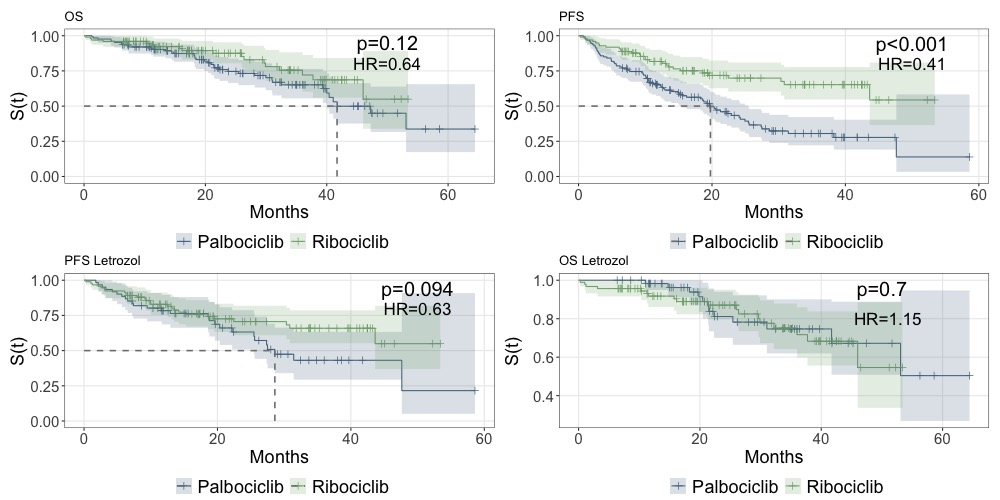
\includegraphics[scale=0.45]{figures/interest_curve_both.jpeg}%

\end{figure}


We then compared both with a cox regression, where OS shows no significant difference between palbociclib and ribociclib but a significantly better PFS for ribociclib (figure \ref*{tab:cox}) HR 0.60 [95\%CI 0.36-0.97] when adjusted to the stage, visceral metastases, age, treatment line, combination and ECOG. This data implies that ribociclib reduces the risk of the disease progression by $~$40\% compared to palbociclib when adjusted for the variables mentioned. The proportional hazards assumption was confirmed with p values all over 0.10.
\begin{table}[ht]
  \centering
  \caption{Cox Regression with palbociclib and Ribociclib - Progression Free Survival and Overall Survival}\label{tab:cox} 
  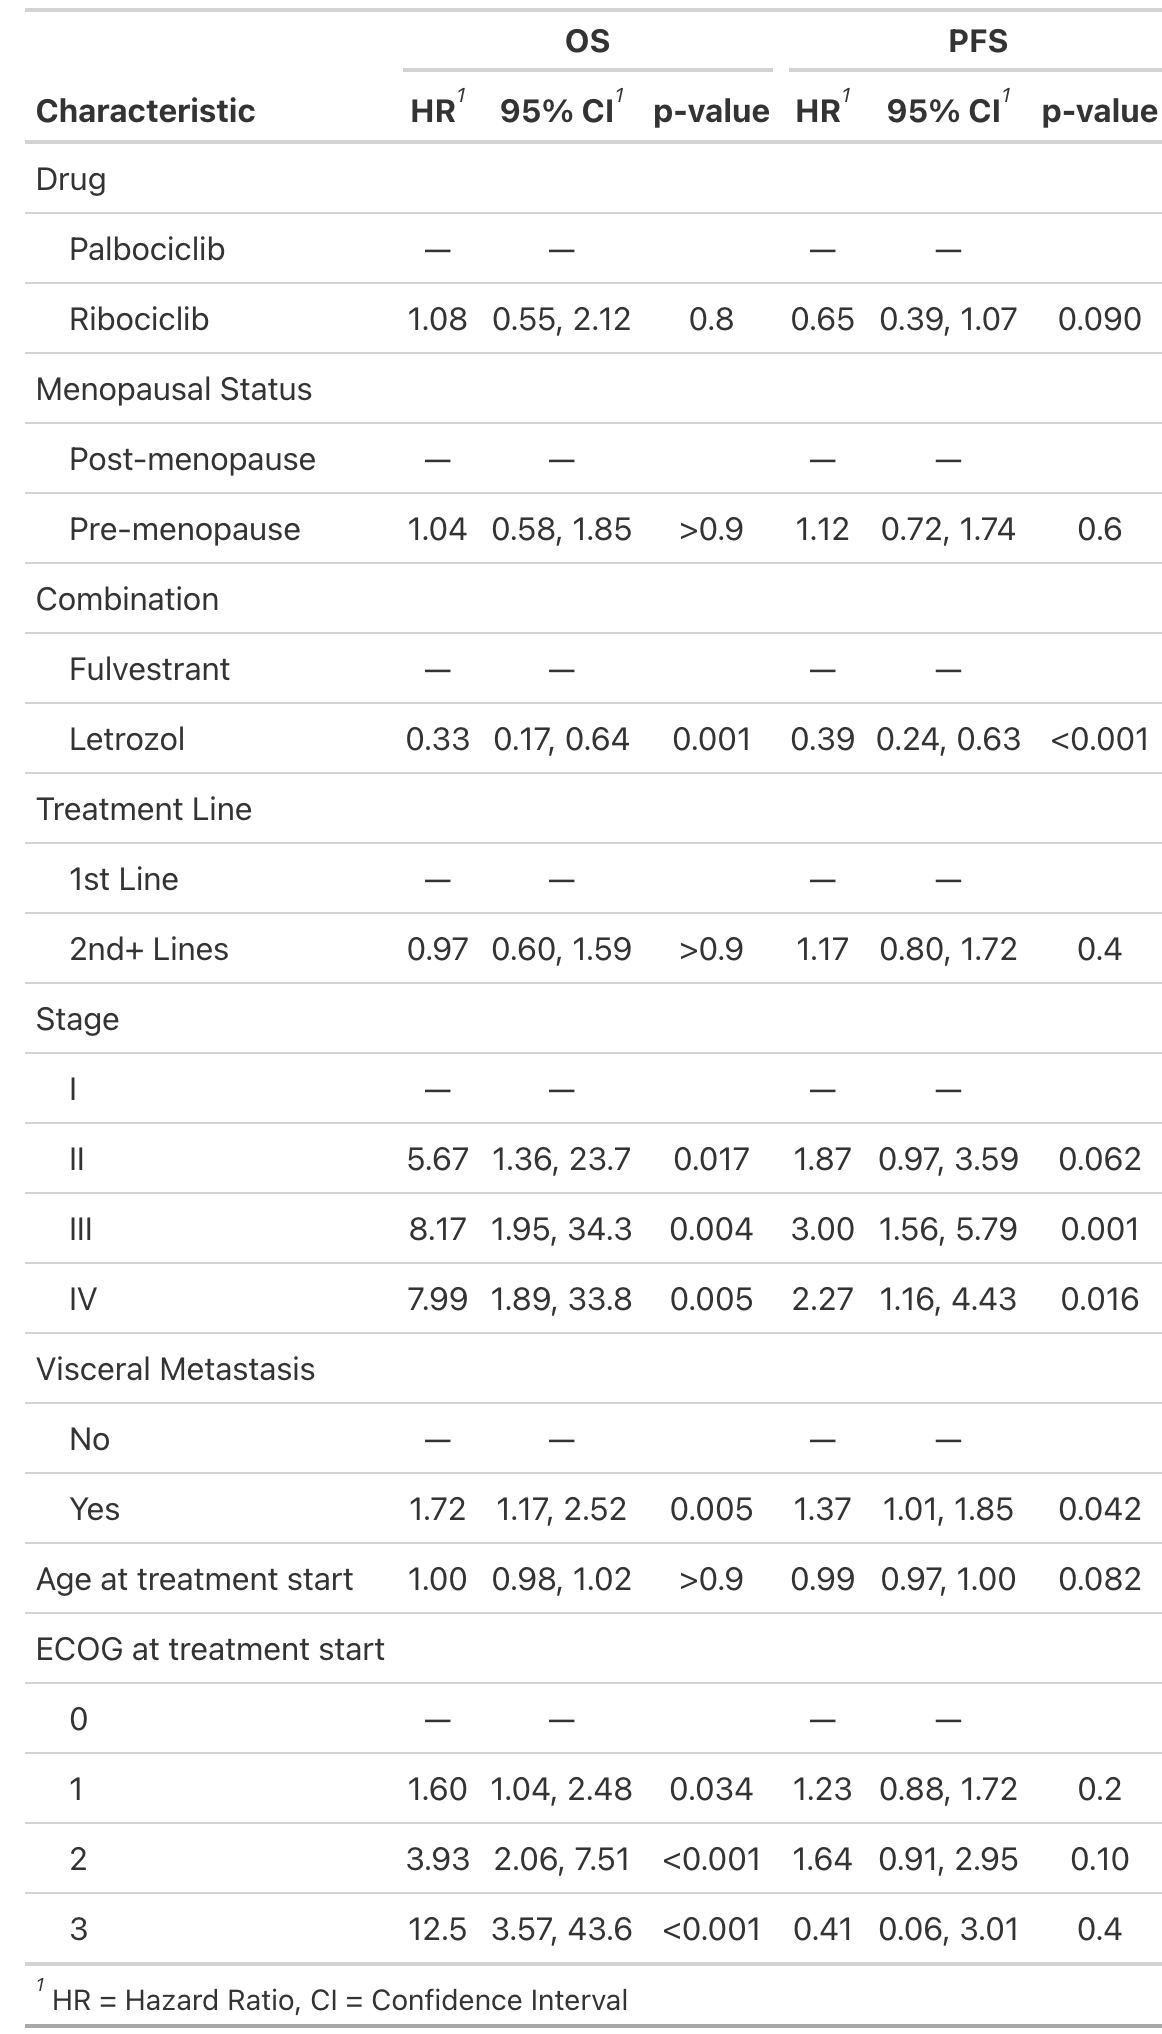
\includegraphics[scale=0.20]{figures/cox_both.png}%

\end{table}

When comparing endocrine therapy with CDK4/6 inhibitors as first-line treatment (figure \ref*{fig:grouped}), we see that only Ribociclib is significantly better in terms of PFS and OS (p-value $\le$ 0.001). When comparing palbociclib as the first line, we see that there is no significant difference in terms of PFS and OS (p=0.6 and 0.47).
We also applied the same analysis as above, comparing only the letrozol combination with letrozol alone. We found that both ribociclib and palbociclib are significantly better in terms of PFS (HR 0.51 for palbociclib and 0.28 for ribociclib).
\begin{figure}[ht]
  \centering

  \caption{Survival curves (OS and PFS) comparing endocrine therapy (ET) to CDK4/6 inhibitors as 1st line. p values shown as pairwise vs. ET. }\label{fig:grouped} 
  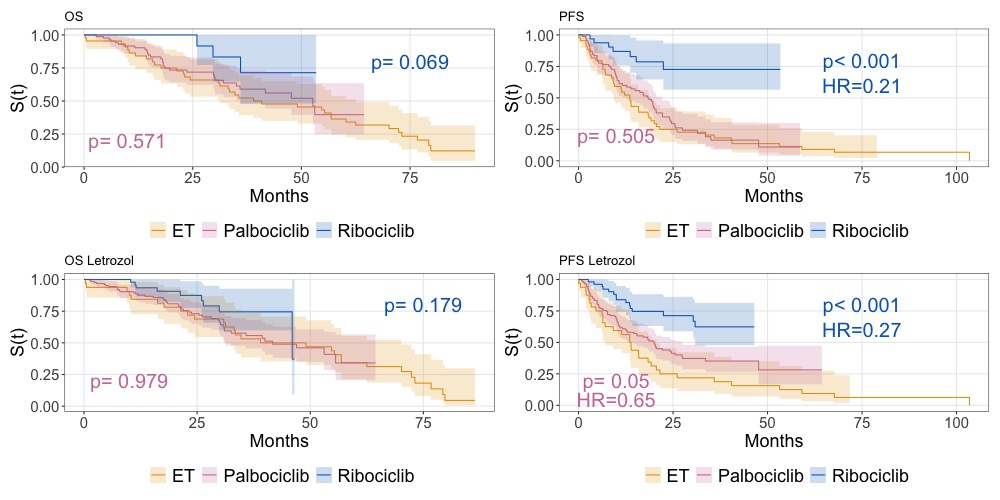
\includegraphics[scale=0.42]{figures/grouped_curve_both.jpeg}%

\end{figure}

When comparing palbociclib and ribociclib adjusted for ATE weights, we found a different scenario from previous assessments. There is a significant difference between the two in terms of OS and PFS (figure \ref*{fig:propensity}). We calculated the weights taking into account stage, age at treatment start, treatment line, and ECOG.

\begin{figure}[ht]
  \centering

  \caption{Comparison of palbociclib and ribociclib survival curves adjusted for propensity scores  }\label{fig:propensity} 
  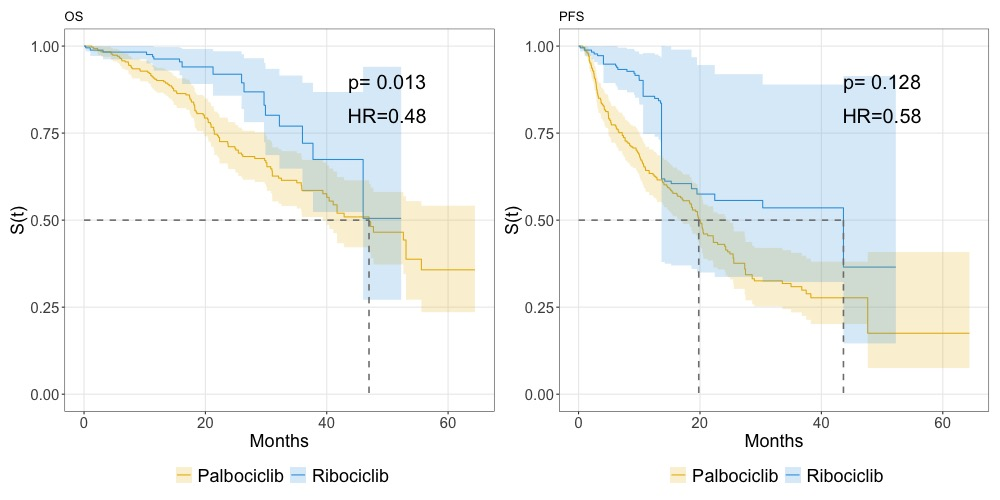
\includegraphics[scale=0.42]{figures/propensity_score_both.jpeg}%

\end{figure}

The Cox regression adjusted for weights shows that ribociclib is not significantly different from palbociclib for OS. The HR for PFS is 0.54 [0.31-0.94;p=0.029], implying that ribociclib reduces the risk of the disease progression by $\sim$50\% compared to palbociclib when adjusted to the stage, combination drug, treatment line, visceral metastasis, age, and ECOG. Proportional hazard assumptions are confirmed as well.